\documentclass[a4paper,
    12pt,
    headings=small,
    ngerman,
    listof=totoc,
    numbers=noenddot]{scrreprt}[2021/11/13]
\usepackage{ifxetex,ifluatex}
\ifcase \ifxetex 1\else\ifluatex 1\else 0\fi\fi\usepackage[utf8]{inputenc}\fi
\usepackage[T1]{fontenc}
\usepackage[ngerman]{babel}
\usepackage[utf8]{inputenc}
\usepackage{setspace}
\onehalfspacing
\usepackage{lmodern}
\usepackage{csquotes}

\usepackage[automark,headsepline=.4pt]{scrlayer-scrpage}
\clearmainofpairofpagestyles
\pagestyle{scrheadings}
\renewcommand*{\chaptermarkformat}{%
	\chaptername~\thechapter\autodot\enskip}
\ihead{\headmark}
\setkomafont{pageheadfoot}{}
\renewcommand*{\sectionmarkformat}{}
\cfoot{\pagemark}
\footskip1cm

\usepackage[left=2.5cm,right=2.5cm,top=3cm,bottom=2.5cm]{geometry}

\usepackage{xcolor, soul}
\definecolor{codebackground}{rgb}{0.95, 0.95, 0.92}
\definecolor{Black}{rgb}{0, 0, 0}

%%% Für Abkürzungen und Abkürzungsverzeichnis %%%
\usepackage[printonlyused,withpage]{acronym}

%%% Für Quotes %%%
\usepackage{url}
\usepackage[ngerman]{varioref}
\usepackage{mwe}
\usepackage{hyperref}% Weil es so in der Frage enthalten war.
 \hypersetup{%draft, 								% no hyperlinking at all (useful in b/w printouts)
    colorlinks=true, breaklinks=true,
    urlcolor=Black, linkcolor=Black, citecolor=Black,
    linktoc=page, %
    bookmarksnumbered, bookmarksopenlevel=1, bookmarksdepth = section,%
    pdfstartview=FitV,
    }
\setlength{\parindent}{0em}

%%% Fuer Glossar
\usepackage[toc]{glossaries}

\usepackage{bookmark}% Weil das hyperref deutlich verbesser.
\usepackage{cleveref}
\crefname{paragraph}{Abschnitt}{Abschnitt}
\crefname{lstlisting}{Listing}{Listings}

\makeglossaries
% \renewcommand*{\glossarysection}[1][]{\chapter{#1}}

%%% Für Textübergreifende Numerierung %%%
\usepackage{enumitem}
\renewcommand{\labelenumi}{\alph{enumi})}

%%% Um PDFs einzubinden %%%
\usepackage{pdfpages}

%%% Um Zahlen mit Einheiten korrekt darstellen %%%
\usepackage{siunitx}
\sisetup{
  locale = DE ,
  detect-all,
  binary-units = true
}

%%% Code schoen darstellen %%%
\usepackage{listings}
\usepackage{listingsutf8}

\lstdefinestyle{MyPythonStyle}{
  frame=tb, % hrule above and below
  keepspaces=true,
  breaklines=true,
  columns=flexible,
  basicstyle=\texttt\scriptsize,
  escapeinside={(*@}{@*)}, % for escaping
  backgroundcolor=\color{codebackground},
  showstringspaces=false,
  language=Python,
  keywordstyle=\color{blue},
  stringstyle=\color{red},
  commentstyle=\color{teal},
  numbers=left, % {none, left, right}
  firstnumber=1,
  numberstyle=\scriptsize\color{black},
  numbersep=5pt,
  xleftmargin=5.0ex,
  gobble=-4
}

\lstdefinelanguage{docker}{
  frame=tb, % hrule above and below
  keepspaces=true,
  breaklines=true,
  columns=flexible,
  basicstyle=\texttt\scriptsize,
  keywords={FROM, RUN, COPY, ADD, ENTRYPOINT, CMD,  ENV, ARG, WORKDIR, EXPOSE, LABEL, USER, VOLUME, STOPSIGNAL, ONBUILD, MAINTAINER},
  keywordstyle=\color{blue}\bfseries,
  identifierstyle=\color{black},
  sensitive=false,
  comment=[l]{\#},
  commentstyle=\color{purple}\ttfamily,
  stringstyle=\color{red}\ttfamily,
  morestring=[b]',
  morestring=[b]",
  numbers=left, % {none, left, right}
  firstnumber=1,
  numberstyle=\scriptsize\color{black},
  numbersep=5pt,
  xleftmargin=5.0ex,
  gobble=0
}

\lstdefinelanguage{docker-compose}{
  frame=tb, % hrule above and below
  keepspaces=true,
  breaklines=true,
  columns=flexible,
  basicstyle=\texttt\scriptsize,
  keywords={image, environment, ports, container_name, ports, volumes, links},
  keywordstyle=\color{blue}\bfseries,
  identifierstyle=\color{black},
  sensitive=false,
  comment=[l]{\#},
  commentstyle=\color{purple}\ttfamily,
  stringstyle=\color{red}\ttfamily,
  morestring=[b]',
  morestring=[b]",
  numbers=left, % {none, left, right}
  firstnumber=1,
  numberstyle=\scriptsize\color{black},
  numbersep=5pt,
  xleftmargin=5.0ex,
  gobble=0
}
\lstdefinelanguage{docker-compose-2}{
  frame=tb, % hrule above and below
  keepspaces=true,
  breaklines=true,
  columns=flexible,
  basicstyle=\texttt\scriptsize,
  keywords={version, volumes, services},
  keywordstyle=\color{blue}\bfseries,
  keywords=[2]{image, environment, ports, container_name, ports, links, build},
  keywordstyle=[2]\color{olive}\bfseries,
  identifierstyle=\color{black},
  sensitive=false,
  comment=[l]{\#},
  commentstyle=\color{purple}\ttfamily,
  stringstyle=\color{red}\ttfamily,
  morestring=[b]',
  morestring=[b]",
  numbers=left, % {none, left, right}
  firstnumber=1,
  numberstyle=\scriptsize\color{black},
  numbersep=5pt,
  xleftmargin=5.0ex,
  gobble=0
}

\lstset{basicstyle=\ttfamily,
  showstringspaces=false,
  commentstyle=\color{red},
  keywordstyle=\color{blue},
  inputencoding=utf8,
  extendedchars=true
}

%%% Korrekte darstellung fuer Sonderzeichen im Code
\lstset{literate=%
    {Ö}{{\"O}}1
    {Ä}{{\"A}}1
    {Ü}{{\"U}}1
    {ß}{{\ss}}1
    {ü}{{\"u}}1
    {ä}{{\"a}}1
    {ö}{{\"o}}1
    {~}{{\textasciitilde}}1
}


%%% Verzeichnisse im Anhang %%%
\DeclareNewTOC[%
  owner=\jobname,
  listname={Inhalt des Anhangs},% Titel des Verzeichnisses
]{atoc}% Dateierweiterung (a=appendix, toc=table of contents)
\DeclareNewTOC[%
  listname={Abbildungen im Anhang},% Titel des Verzeichnisses
]{alof}% Dateierweiterung (a=appendix, lof=list of figures)
\DeclareNewTOC[%
  listname={Tabellen im Anhang},% Titel des Verzeichnisses
]{alot}% Dateierweiterung (a=appendix, lot=list of tables)
 
\makeatletter
\newcommand*{\useappendixtocs}{%
  \renewcommand*{\ext@toc}{atoc}%
  \scr@ifundefinedorrelax{hypersetup}{}{% damit es auch ohne hyperref funktioniert
    \hypersetup{bookmarkstype=atoc}%
  }%
  \renewcommand*{\ext@figure}{alof}%
  \renewcommand*{\ext@table}{alot}%
}
\newcommand*{\usestandardtocs}{%
  \renewcommand*{\ext@toc}{toc}%
  \scr@ifundefinedorrelax{hypersetup}{}{% damit es auch ohne hyperref funktioniert
    \hypersetup{bookmarkstype=toc}%
  }%
  \renewcommand*{\ext@figure}{lof}%
  \renewcommand*{\ext@table}{lot}%
}
\scr@ifundefinedorrelax{ext@toc}{%
  \newcommand*{\ext@toc}{toc}
  \renewcommand{\addtocentrydefault}[3]{%
    \expandafter\tocbasic@addxcontentsline\expandafter{\ext@toc}{#1}{#2}{#3}%
  }
}{}
\makeatother
 
\usepackage{xpatch}
\xapptocmd\appendix{%
  \addpart{\appendixname}
  \useappendixtocs
}{}{}

%%% Alles bzgl. des Literaturverzeichnisses
\usepackage[bibencoding=utf8,
			sortlocale=de,
			style=numeric,
			pagetracker=true,
			autocite=inline,
			backrefstyle=three+,
			date=short,
			sorting=nty,
			backend=biber]{biblatex}
\bibliography{Literaturverzeichnis}

%%% urldate in eckigen Klammern %%%
\DeclareFieldFormat{urldate}{\mkbibbrackets{#1}}
%%% URL: = Verfügbar unter: %%%
\DeclareFieldFormat{url}{{Verfügbar unter:}\space\url{#1}}
%%% Abstand zwischen den Literaturangaben %%%
\setlength{\bibitemsep}{1.3em}
%%% statt und ein & %%%
\renewcommand*{\finalnamedelim}{\space\&\space}
%%% Nachname, Vorname, immer %%%
\DeclareNameAlias{sortname}{last-first}

\title{Die hard- und softwaretechnische Implementierung eines CO$_2$-Sensors zur Messung der Raumluftqualität}
\author{Julius Caesar, Péter Egermann, Paul Görtler, Johannes Leyrer}
\date{\today}

\begin{document}
\maketitle

\newpage

\tableofcontents

\newpage

\chapter*{Abkürzungsverzeichnis}

\begin{acronym}[DGUV]
  \acro{API}{Application Programming Interface}
  \acro{ASR}{Technische Regeln für Arbeitsstätten}
  \acro{DGUV}{Deutsche Gesetzliche Unfallversicherung}
  \acro{HIDs}{Human Interface Devices}
  \acro{ppm}{parts per million}
  \acro{UBA}{Umweltbundesamt}
  \acro{ZNS}{Zentralnervensystem}
\end{acronym}

%%% Glossareintraege
\newglossaryentry{backend}
{
  name=backend,
  description={Als Backend wird der Teil eines IT-Systems bezeichnet, der sich mit der Datenverarbeitung im Hintergrund beschäftigt – der Data Layer. Der Begriff dient der Unterteilung bei komplexeren Softwarestrukturen. Die Schreibweise wird vom Duden nicht genau vorgegeben. \autocite{backend_definition}}
}
\newglossaryentry{frontend}
{
  name=frontend,
  description={Der Begriff Frontend dient bei komplexeren Softwarestrukturen der Unterteilung. Bei einem IT-System bezeichnet das Frontend die Presentation Layer, also den Teil eines IT-Systems, der näher am Anwender ist. \autocite{frontend_definition}}
}
\newglossaryentry{hidraw}
{
  name=hidraw,
  description={Der hidraw-Treiber bietet eine Rohschnittstelle zu USB- und Bluetooth-\ac{HIDs}.}
}
\newglossaryentry{Python}
{
  name=Python,
  description={ist eine plattformunabhängige, multiparadigmatische, stark und dynamisch typisierte Programmiersprache.
      Die Programmiersprache zeichnet sich besonders durch ihre Trivialität und vielseitige Einsetzbarkeit aus.
      Python ist eine der meist verbreiteten Programmiersprachen weltweit.
      Die Weiterentwicklung der Programmiersprache wird durch die Python Software Foundation und den ursprünglichen Entwickler Guido van Rossum durchgeführt. \autocite{python}}
}
\newglossaryentry{Docker}
{
  name=Docker,
  description={ist eine freie Softwareplattform der Docker, Inc. Das Ziel von Docker ist es, das Erstellen, Testen und Bereitstellen von Software im wesentlich zu beschleunigen.
      Mit Docker können Softwarepakete, sogenannte Container, erstellt werden. Diese gewährleisten eine Trennung und Verwaltung der lokalen Computerressourcen.
      Die am 13.03.2013 erstmals veröffentlichte Software ist unter anderem für die Betriebssysteme Linux, Microsoft Windows und macOS verfügbar. \autocite{docker_setup} \autocite{docker_install}}
}
\newglossaryentry{docker-compose}
{
  name=docker-compose,
  description={docker-compose ist ein Tool, das entwickelt wurde, um die Definition und gemeinsame Nutzung von Multicontainer-Anwendungen zu erleichtern. Mit Compose kann eine YAML-Datei erstellen werden, um die Dienste zu definieren, und mit einem einzigen Befehl können alle Container in Gang gesetzt oder abgebaut werden. \autocite{docker_install}}
}

\newpage


\chapter{Einleitung}

Im Laufe der Corona-Pandemie und der damit verbundenen Ausgangsbeschränkungen musste man sich zunehmen in Innenräumen aufhalten, um der Verbreitung des Virus entgegenzuwirken. Aus diesem Grund musste man sich zwangsweise mit der Luftqualität im Homeoffice und besonders in Büroräumen auseinandersetzen, um das Gesundheitsrisiko zu minimieren und konzentriert arbeiten zu können. Da die Luftqualität durch Menschen meist nur subjektiv wahrgenommen werden kann, benötigt man dafür eine Messstelle. Da die gesundheitlichen Auswirkungen von schlechter Raumluftqualität ausreichend erforscht sind, existieren genügend konkrete Werte zur Orientierung.

Diese Arbeit soll einen Überblick darüber geben, welche medizinischen Risiken durch eine unzureichende Luftqualität entstehen können und welche positiven Auswirkungen eine ausreichende Versorgung mit Frischluft haben kann.

Danach soll ein grober Leitfaden zur Einrichtung eines CO$_2$-Sensors zur Bestimmung der Luftqualität in Arbeitsräumen erstellt werden. Dabei soll über die Anforderungen an die Hardware, die benötigten Komponenten, die Einbindung in das Netzwerk und die Umsetzung der dazugehörigen Software eingegangen werden. Die Arbeit richtet sich dabei hauptsächlich an technisch versierte Leser, welche bereits grundlegende Kenntnisse in den Bereichen Hard- und Software besitzen.


\chapter{CO\texorpdfstring{$_2$}{TEXT}-Grenzwerte und deren Auswirkungen auf den Menschen}\label{chapter:2}

Um sich der Wichtigkeit einer Messung des CO$_2$-Gehaltes in der Atemluft bewusst zu werden, werden in diesem Kapitel die von verschiedenen Institutionen festgelegten CO$_2$-Grenzwerte zusammengefasst.

Weiterhin werden die verschiedenen physiologischen Risiken, die durch einen zu hohen CO$_2$-Gehalt in der Raumluft drohen, vorgestellt. Der CO$_2$-Gehalt wird in \ac{ppm} angegeben.


\section{CO\texorpdfstring{$_2$}{TEXT}-Grenzwerte für eine unbedenkliche Atemluft}

Die \ac{DGUV} veröffentlicht \ac{ASR}, zu diesen gehört auch die \ac{ASR} A3.6 \enquote{Lüftung} \autocite{ASR}, welche sich in Kapitel 4 mit Regelungen zur Luftqualität von Arbeitsplätzen auseinandersetzt.

Wie in \vref{appendix:tab:dguv_table_co2} zu sehen, wird eine generelle CO$_2$-Konzentration von unter \SI{1000}{\ac{ppm}} als ungefährlich eingestuft und fordert keine weiteren Maßnahmen. Bei einer CO$_2$-Konzentration von \si{1000} bis \SI{2000}{\ac{ppm}} wird die Luftqualität als hygienisch auffällig beschrieben, dabei werden bereits Maßnahmen wie bessere Lüftungsmaßnahmen und eine Überprüfung des aktuellen Lüftungsverhalten empfohlen. Ab einer generellen CO$_2$-Konzentration von über \SI{2000}{\ac{ppm}} stuft die \ac{DGUV} die Atemluft als hygienisch inakzeptabel ein, hierbei werden
Gegenmaßnahmen wie eine verstärkte Lüftung bis zur Reduktion der Personenzahl im Raum empfohlen.

Diese Messungen sollen laut der \ac{ASR} A3.6 \autocite{ASR} in einer Höhe von \SI{1.50}{\metre} und einem Abstand von \si{1} bis \SI{2}{\metre} von Wänden erfolgen, mit einer ausreichend großen Distanz zu Personen, damit diese die Messungen nicht direkt durch ihre Atemluft beeinflussen.

Die DIN EN 16798-1 \autocite{din_en_16798} \enquote{Energetische Bewertung von Gebäuden - Lüftung von Gebäuden} \autocite{din_en_16798}, regelt die CO$_2$-Grenzwerte strikter und feingranularer als die \ac{ASR} A3.6 \autocite{ASR}. Wie in \vref{appendix:tab:din_table_co2} wird bei Werten unter \SI{950}{\ac{ppm}} von einer hohen Raumluftqualität gesprochen, von \si{950} bis \SI{1200}{\ac{ppm}} gilt die Raumluftqualität als \enquote{mittlere Raumluftqualität}. CO$_2$-Konzentrationen von \si{1200} bis \SI{1750}{\ac{ppm}} werden als \enquote{Mäßige Raumluftqualität} und Werte über \SI{1750}{\ac{ppm}} als \enquote{Niedrige Raumluftqualität} eingestuft.

Aus den beiden vorgestellten Bewertungen der CO$_2$-Konzentration für die Raumluft kann geschlossen werden, dass die CO$_2$-Konzentration generell nicht über \SI{1000}{\ac{ppm}} steigen sollte, damit die Raumluft eine ausreichend hohe Qualität aufweist.


\section{Physiologische Auswirkungen eines zu hohen CO\texorpdfstring{$_2$}{TEXT}-Gehaltes in der Atemluft}

Eine von Kajtár et al. \autocite{kajtar} durchgeführte Studie hat gezeigt, dass eine höhere CO$_2$-Konzentration zu einer schnelleren Erschöpfung beim Lösen von Aufgaben führt. Dafür sollten zehn Probanden unter verschiedenen CO$_2$-Konzentrationen über einen Zeitraum von jeweils zwei mal 70 Minuten einen Text auf Fehler korrigieren. Dabei wurde festgestellt, dass sich die mentale Leistungsfähigkeit im Gegensatz zu einer akzeptablen CO$_2$-Konzentration von \SI{600}{\ac{ppm}} verringert. Die Messung von physiologischen Parametern der Probanden zeigte außerdem, dass das Lösen von Denkaufgaben dadurch ebenfalls anstrengender wird. Bei einem Aufenthalt von zwei bis drei Stunden in einem geschlossenen Raum führte eine CO$_2$-Konzentration von \SI{3000}{\ac{ppm}} zu einer verringerten Konzentrationsfähigkeit.

Zhang et al. \autocite{zhang} kamen in einer Studie mit 15 Probanden und Probandinnen zu der Erkenntnis, dass eine erhöhte CO$_2$-Konzentration in der Atemluft zu einer stark verringerten Leistungsfähigkeit beim Lösen von Denkaufgaben führt. Dafür wurden die  Teilnehmenden verschiedenen CO$_2$-Konzentrationen (\si{1500}, \si{3500} und \SI{5000}{\ac{ppm}}) ausgesetzt, während sie verschiedene Aufgaben lösen mussten. Der Abfall der Leistungsfähigkeit wurde dabei erst bei der Veränderung der CO$_2$-Konzentration von \SI{1500}{\ac{ppm}} auf \SI{3500}{\ac{ppm}} festgestellt. Bei einem weiteren Anstieg des Wertes auf \SI{5000}{\ac{ppm}} wurden keine weiteren Veränderung der mentalen Leistungsfähigkeit festgestellt.

Bei einer Studie, die von Myhrvold et al. \autocite{myhrvold} mit 548 Schüler*innen durchgeführt wurde, wurden die Auswirkungen auf den Körper, speziell auf das \ac{ZNS}, die Haut und Schleimhaut untersucht. Während bei dieser Studie die Auswirkungen auf die mentale Leistungsfähigkeit nicht signifikant auffällig waren, wirkte sich eine CO$_2$-Konzentration von über \SI{1500}{\ac{ppm}} negativ auf das körperliche Wohlbefinden aus. Dabei wurden unter anderem Symptome wie Kopfschmerzen, Müdigkeit, Konzentrationsschwäche und Hustenanfälle festgestellt.

Ein ähnliches Ergebnis erzielt auch eine von Tiesler et al. \autocite{tiesler} durchgeführte Studie. Dafür wurde der CO$_2$-Gehalt der Atemluft in den Klassenräumen von 16 Klassen aus drei verschiedenen Bremer Schulen und dessen Wirkung auf die Schüler*innen untersucht. Dabei wurde festgestellt, dass sich regelmäßiges Lüften, um die CO$_2$-Konzentration zu senken, positiv auf das Wohlbefinden der  Teilnehmenden auswirkt. Der zu erreichende Zielwert durch das erhöhte Lüftungsintervall lag dabei unter \si{1000} bzw. \SI{1500}{\ac{ppm}}, die vorher  erreichten Werte nach einer Doppelstunde erreichten bis zu \SI{4000}{\ac{ppm}}. Die Schüler*innen berichteten in Befragungen von einer verbesserten Aufmerksamkeit, welche sich wahrscheinlich auf die geringere CO$_2$-Konzentration in der Raumluft zurückführen lässt.



\chapter{Hardwaretechnische Umsetzung}


\section{Technische Anforderungen an die benötigte Hardware}

Um einen CO$_2$-Monitor betreiben zu können werden ein Computer und ein CO$_2$-Sensor benötigt. Die Mindestanforderungen an den Computer sind 512MB Arbeitsspeicher, einen ARM Cortex-A53 Quad-Core 1GHz 64-bit Prozessor und mindestens einem USB Type A Anschluss. Diese Werte sind die Mindestanforderungen von einem minimalen Linux Betriebssystem, welches benötigt wird um die Softwareanforderungen zu erfüllen.

Der CO$_2$-Sensor sollte ein Messbereich von \SI{0}{ppm} bis einschließlich \SI{2000}{ppm} vorweisen. Mit dieser Spannweite können die in \vref{chapter:2} vorgestellten Werte für die Aussage über Luftqualität gemessen und aufgezeichnet werden.


\section{Überblick über die verwendete Hardware}

Für die Verwendung der Programme rund um den CO$_2$-Monitor wird folgende Hardware benötigt:

\begin{itemize}
  \item Raspberry Pi 3 Model B+
  \item TFA-Dostmann CO$_2$-Monitor AIRCO2NTROL MINI
\end{itemize}

Der Raspberry Pi ist ein Minicomputer auf einer nur Scheckkarten-großen Platine, der sich vielfältig erweitern lässt.
Er wurde ursprünglich zu Lern- und Demonstrationszwecken entwickelt, eignet sich aber auch für die
Realisierung verschiedener privater oder professioneller Anwendungen.

Mit dem CO$_2$-Monitor AIRCO2NTROL MINI kann die Luft in Räumen,
in denen sich Personen aufhalten, z.B. Schulen, Büros, öffentliche Einrichtungen, kontrolliert werden. Der Monitor zeigt auf einem Display den CO$_2$-Gehalt der Raumluft im Wechsel mit der Temperatur an. Eine farbige Ampelanzeige neben dem Display wechselt je nach Luftqualität von Grün über Gelb zu Rot.



\chapter{Softwaretechnische Umsetzung}


\section{Benötigte Software}

Um die Programme rund um den CO$_2$-Monitor in Betrieb nehmen zu können, wird folgende Software benötigt:

\begin{itemize}
  \item PiOS mit mitgelieferter Standardsoftware
  \item \gls{Docker}
  \item \gls{docker-compose}
\end{itemize}

Ist die benötigte Software installiert und eingerichtet, kann mit der Implementierung der Auslese- und Verarbeitungssoftware begonnen werden. Alle in den folgenden Kapiteln genannten Softwarekomponenten sind auf GitHub zu finden.


\section{Zusammenspiel der Softwarekomponenten}

Die Daten des CO$_2$-Sensors werden persistent gespeichert, damit die Werte abrufbar sind und auch über längere Zeiträume ausgewertet werden können. Dafür werden die CO$_2$- und Temperaturwerte mittels einer Software-Komponente zum Auslesen der Daten an ein \gls{backend} gesendet und gespeichert. Diese Daten können dann mittels eines \gls{frontend}s angezeigt werden. Diese Verknüpfung der Software-Komponenten ist in \vref{fig:Verbundplan} zu sehen.

\begin{figure}[htbp]
  \centering
  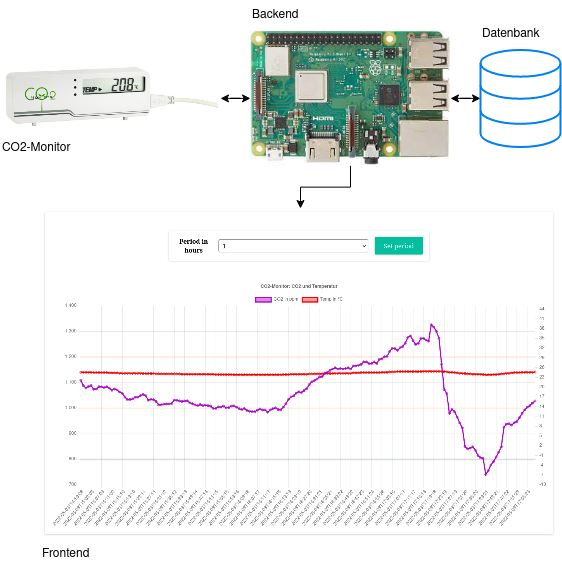
\includegraphics[width=0.9\textwidth]{pictures/SoftwareZusammenspiel.png}
  \caption{Verbundplan der Komponenten}
  \label{fig:Verbundplan}
\end{figure}


\section{Aufbau und Einrichten der Software}

\subsection{Aufbau und Einrichten des \gls{backend}s}

Die zentrale Stelle, an der Daten eingehen, gespeichert und abgerufen werden können, wird mittels der \textit{CO2MonitorAPI} realisiert. Diese ist in \gls{Python} geschrieben und verwendet FastAPI als Grundlage für das Bereitstellen einer API. Um das Bereitstellen der Anwendung und deren  Isolierung vom Betriebssystem zu erleichtern, wird \gls{Docker} als Containervirtualisierungssoftware eingesetzt.

Nachdem die Anwendung von GitHub bezogen wurde, müssen noch Konfigurationswerte angepasst werden. Beispielsweise muss der Port festgelegt werden, auf dem die \ac{API} erreichbar sein soll. Hierfür kann in der \texttt{docker-compose.yml}-Datei besagter Port angegeben werden, welcher dem \gls{frontend} und dem CO2Reader Zugang zur \gls{backend}-Logik erlaubt, um Daten abzuspeichern und abzurufen.

Durch das Öffnen eines Terminal-Fensters im Ordner der \ac{API} und der Eingabe des Befehls

\begin{lstlisting}[language=Bash]
  docker-compose -f docker-compose.yml up -d
\end{lstlisting}

wird die Anwendung gestartet. Der \gls{Docker}-Container läuft ab jetzt im Hintergrund und wartet auf Speicher- oder Abrufbefehle. Ob die Applikation richtig funktioniert kann mittels

\begin{lstlisting}
  IpAdresseDesPis:angegebenerPort/api/test
\end{lstlisting}

getestet werden.


\subsection{Aufbau und Einrichten der Lese-Software}

Die Daten des CO$_2$-Sensors werden mittels der USB-Schnittstelle ausgelesen. Diese Lesesoftware ist in \gls{Python} geschrieben und nutzt die CO2Meter-Bibliothek von Vladimir Filimonov.
\autocite{github_co2meter}

Dazu muss die \texttt{docker-compose.yml}-Datei des \textit{Readers} angepasst werden. Um den richtigen USB-Port in die Datei schreiben zu können, können alle angeschlossenen USB-Geräte mit dem in \cref{lst:bash:hidraw} zu sehenden Bash-Script angezeigt und die \gls{hidraw}-Id des Geräts \textit{Holtek Semiconductor, Inc. USB-zyTemp} ausgelesen werden. \autocite{get_usb_hidraw}

\begin{lstlisting}[language=docker-compose-2,caption={Bash-Script zum Erkennen der \gls{hidraw}-Id},breaklines=true,label={lst:bash:hidraw}]
  #!/bin/bash

  FILES=/dev/hidraw*
  for f in $FILES
  do
    FILE=${f##*/}
    DEVICE="$(cat /sys/class/hidraw/${FILE}/device/uevent | grep HID_NAME | cut -d '=' -f2)"
    printf "%s \t %s\n" $FILE "$DEVICE"
  done
\end{lstlisting}

Ist der USB-Port bestimmt, kann der Teil vor dem Doppelpunkt der \texttt{devices}, in diesem Fall \enquote{\texttt{/dev/hidraw0}}, mit dem ausgelesenen Port ersetzt werden, zu sehen in \vref{lst:compose:hidraw}.

\begin{lstlisting}[language=docker-compose-2,caption={Anpassen des USB-Ports in der docker-compose.yml},breaklines=true,label={lst:compose:hidraw}]
  ...
    devices:
      - /dev/hidraw0:/dev/hidraw16
  ...
\end{lstlisting}

Soll der \textit{Reader} auf einem anderen Gerät als die \ac{API} ausgeführt werden, muss die \texttt{co2Reader.ini}-Datei angepasst werden. Diese ist in \texttt{app/co2Reader.ini} zu finden. Hier muss die IP-Adresse der \ac{API} anstelle der bestehenden IP-Adresse angegeben werden. Auch kann hier der Ort, an dem sich der Sensor befindet, eingetragen werden.

Nach dem Abspeichern der Datei kann ein Terminal-Fenster im Ordner des \textit{Readers} geöffnet werden und mittels

\begin{lstlisting}[language=Bash]
  docker-compose -f docker-compose.yml up -d
\end{lstlisting}

die Anwendung gestartet werden. Der \gls{Docker}-Container läuft ab jetzt im Hintergrund, liest die Daten des Sensors aus und schickt diese an die angegebene IP-Adresse der \ac{API}.

\subsection{Aufbau und Einrichten des Frontends}

Um die Daten ansehnlich darstellen zu können, kann ein \gls{frontend} eingebunden werden. Das hier verwendete \gls{frontend} ist mit React \autocite{reactjs} und ChartsJs \autocite{chart.js} umgesetzt worden. Ein Beispiel der Datenvisualisierung ist in \vref{fig:frontend} zu sehen.

\begin{figure}[htbp]
  \centering
  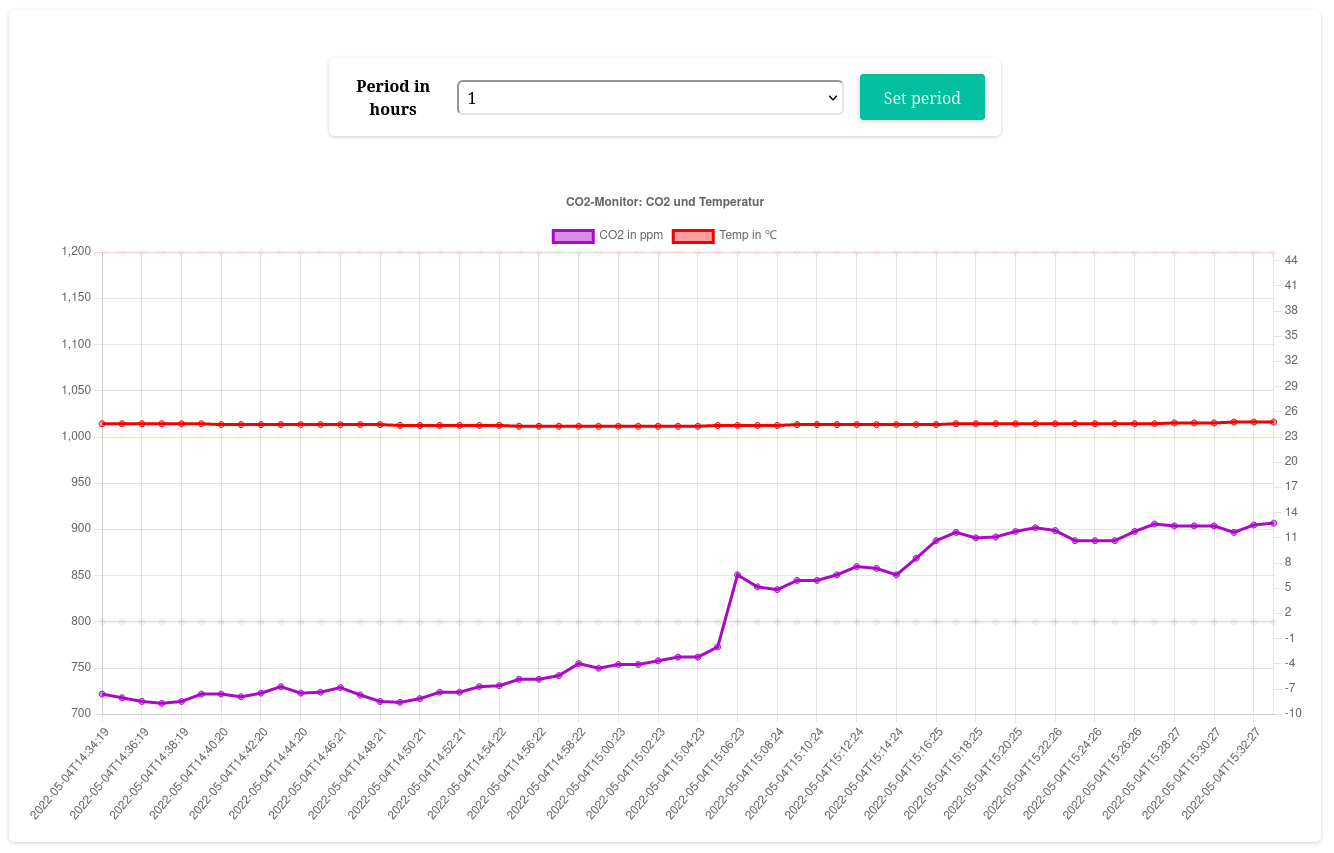
\includegraphics[width=0.95\textwidth]{pictures/Frontend.png}
  \caption{Datenvisualisierung mittels \gls{frontend}}
  \label{fig:frontend}
\end{figure}

Nachdem das \gls{frontend} bezogen wurde muss die \texttt{docker-compose.yml}-Datei angepasst werden. In dieser Datei muss die IP-Adresse der \texttt{REACT\_APP\_API\_URL} mit der IP des Raspberry Pis, auf dem die \ac{API} läuft ausgetauscht werden, zu sehen in \vref{lst:compose:react_ip}.

Der ausgehende Port, von dem das \gls{frontend} am Ende erreichbar ist, kann ebenfalls angepasst werden. Hierzu muss lediglich der ports-Abschnitt verändert werden, ebenfalls zu sehen in \vref{lst:compose:react_ip}. Hier muss der Port vor dem Doppelpunkt auf den gewünschten Port gesetzt werden.

\begin{lstlisting}[language=docker-compose-2,caption={Anpassen der \ac{API}-IP und des Ports in der docker-compose.yml},breaklines=true,label={lst:compose:react_ip}]
  ...
  environment:
    REACT_APP_API_URL: http://192.168.178.33:8008/api/
  ports:
    - 3000:3000
  ...
\end{lstlisting}

Mit dem Öffnen eines Terminal-Fensters im Ordner des \gls{frontend}s und mittels

\begin{lstlisting}[language=Bash]
  docker-compose -f docker-compose.yml up -d
\end{lstlisting}

wird Anwendung gestartet. Der \gls{Docker}-Container läuft ab jetzt im Hintergrund und kann mittels der IP-Adresse des ausführenden Gerätes sowie dem in der \texttt{docker-compose.yml}-Datei angegebenen Port aufgerufen werden.



\chapter{Zusammenfassung}
Eine zu hohe CO$_2$-Konzentration in der Raumluft mindert die Konzentrationsfähigkeit, die Produktivität und das körperliche Wohlbefinden der in diesen Räumen arbeitenden Menschen. Die von der \ac{DGUV} \ac{ASR} A3.6 \autocite{ASR} und der DIN EN 16798-1 \autocite{din_en_16798} festgelegten Grenzwerte für den CO$_2$-Gehalt der Raumluft decken sich in etwa mit den durch verschiedene Studien belegten Grenzwerten und bilden damit eine aussagekräftige Grundlage für die Einschätzung der Raumluftqualität. Die Einrichtung eines CO$_2$-Monitors mittels Raspberry-Pi und eines CO$_2$-Sensors ist eine relativ kostengünstige und mit etwas Vorwissen auch einfach zu implementierende Möglichkeit, den CO$_2$-Gehalt der Raumluft zu bestimmen. Diese Messungen sollte vor allem in Büros und Klassenräumen stattfinden, da dort generell viele Menschen auf engem Raum arbeiten und ihre Leistung möglichst nicht durch ein schlechtes Raumklima vermindert werden sollte.



\newpage

%%% Abbildungsverzeichnis
\listoffigures
%%% Codeverzeichnis
\lstlistoflistings
%%% Glossar
\printglossary
% \printglossaries
%%% Literaturverzeichnis
\printbibliography

\newpage

\appendix
\ihead{Anhang}

\tableofcontents
%%% Abbildungsverzeichnis
% \listoffigures
%%% Tabellenverzeichnis
\listoftables
%%% Codeverzeichnis
% \lstlistoflistings

% \begin{figure}[h!]
%   \centering
%   \includegraphics[angle=90,origin=c,width=0.75\textwidth]{data/Gantt.png}
%   \caption{Gantt-Diagramm}
%   \label{fig:Gantt}
% \end{figure}


\chapter{Bewertung der CO\texorpdfstring{$_2$}{TEXT} Konzentration in der Raumluft nach \ac{DGUV} \ac{ASR} A3.6}

\begin{table}[htbp]
  \centering
  \renewcommand{\arraystretch}{1.25}
  \caption{Bewertung der CO$_2$ Konzentration in der Raumluft nach \ac{DGUV} \ac{ASR} A3.6 \autocite{ASR}}
  \begin{tabular}{c|p{0.6\textwidth}}
    CO$_2$-Konzentration in \ac{ppm} & Maßnahmen                                                                                                                  \\
    \hline
    $<$1000                          & $\bullet$ Keine weiteren Maßnahmen (sofern durch die Raumnutzung kein Konzentrationsanstieg über 1000 ppm zu erwarten ist) \\
    \hline
    1000-2000                        & $\bullet$ Lüftungsverhalten überprüfen und verbessern                                                                      \\
                                     & $\bullet$ Lüftungsplan aufstellen (z. B. Verantwortlichkeiten festlegen)                                                   \\
                                     & $\bullet$ Lüftungsmaßnahme (z. B. Außenluftvolumenstrom oder Luftwechsel erhöhen)                                          \\
    \hline
    $>$2000                          & $\bullet$ weitergehende Maßnahmen erforderlich (z. B. verstärkte Lüftung, Reduzierung der Personenzahl im Raum)            \\
  \end{tabular}
  \label{appendix:tab:dguv_table_co2}
\end{table}

\chapter{Bewertung der CO\texorpdfstring{$_2$}{TEXT} Konzentration in der Raumluft nach DIN EN 16798-1}

\begin{table}[htbp]
  \centering
  \renewcommand{\arraystretch}{1.25}
  \caption{Bewertung der CO$_2$ Konzentration in der Raumluft nach DIN EN 16798-1 \autocite{din_en_16798}}
  \begin{tabular}{c|p{0.6\textwidth}}
    CO$_2$-Konzentration in \ac{ppm} & Beschreibung              \\
    \hline
    $<$950                           & Hohe Raumluftqualität     \\
    950-1200                         & Mittlere Raumluftqualität \\
    1200-1750                        & Mäßige Raumluftqualität   \\
    $>$1750                          & Niedrige Raumluftqualität \\
  \end{tabular}
  \label{appendix:tab:din_table_co2}
\end{table}

\end{document}
